\subsection{Source Injection}
\label{sec:source_injection}

The \texttt{source\_injection} package contains tools designed to assist in the injection of synthetic sources into scientific imaging.
Source injection is a powerful tool for testing the algorithmic performance of the LSST Science Pipelines, generating measurements on synthetic sources where the truth is known and facilitating subsequent quality assurance checks.
Synthetic source generation and injection capability is provided by the \textsc{GalSim} software package \citep{2015A&C....10..121R}.
An example showcasing the injection of a series of synthetic Sérsic sources into an HSC i-band image is shown in Figure \ref{fig:source_injection_example}.

\begin{figure}
    \centering
    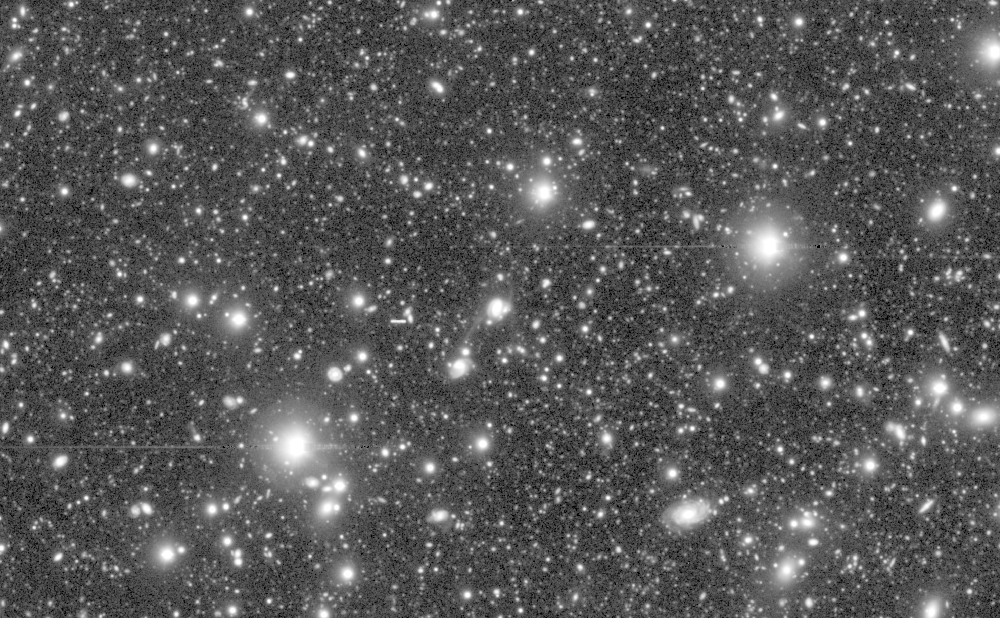
\includegraphics[width=\linewidth]{figures/t9813p42i_zoom_sersic_pre_injection}
    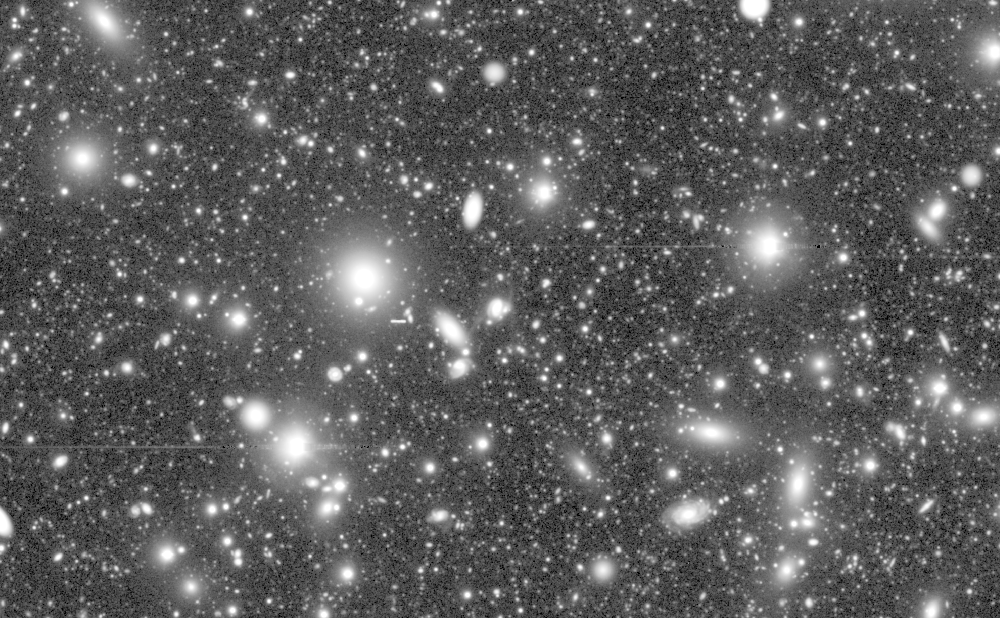
\includegraphics[width=\linewidth]{figures/t9813p42i_zoom_sersic_post_injection}
    \caption{
        An HSC i-band cutout from tract 9813, patch 42, showing before (top) and after (bottom) the injection of a series of synthetic Sérsic sources.
        Images are ~100 arcseconds on the short axis, log scaled across the central 99.5\% flux range, and smoothed with a Gaussian kernel of FWHM 3 pixels.
    }
    \label{fig:source_injection_example}
\end{figure}

Synthetic sources can be injected into any imaging data product output by the LSST Science Pipelines, including visit-level exposure-type or visit-type datasets (i.e., datasets with the dimension \texttt{exposure} or \texttt{visit}), or into a coadd-level coadded dataset.
These injection tasks are defined in \texttt{ExposureInjectTask}, \texttt{VisitInjectTask} and \texttt{CoaddInjectTask}, respectively.
Each task operates similarly: read in an injection catalog containing the parameters of the sources to be injected, generate sources using \textsc{GalSim}, and inject them into the input image.
An additonal mask plane (\texttt{INJECTED} by default) is appended to the image mask to identify pixels which have been touched by injected sources.
Optional modifications to the noise profiles of injected sources and the variance plane of the image can also be performed.

With \textsc{GalSim} we have the capacity to generate synthetic sources of varying profile types, including Gaussian, exponential and Sérsic profiles \citep{1963BAAA....6...41S, 1968adga.book.....S}, each convolved with the local PSF.
We also have the option to inject scaled versions of the PSF model itself in order to simulate stars.
If preferred, a pre-generated FITS image of a source can be injected instead of a model generated by \textsc{GalSim}, allowing for the injection of complex sources or postage stamp cutouts of real data.

Alongside the primary injection tasks, a suite of helper tools are also provided to optionally assist in the generation of synthetic source catalogs and injection pipelines.
Fully qualified source injection pipeline definition YAML files are normally constructed using an existing pipeline as a baseline reference.
A user specifies which dataset type they would like to inject synthetic sources into, and the \texttt{source\_injection} package generates a new pipeline definition YAML file that includes the correctly configured source injection task.
By default, all tasks in the pipeline downstream of the point at which source injection occurs are modified such that their connection names are prefixed with \texttt{injected\_}.
This ensures that an injected dataset is not confused with the original dataset when stored together in a common collection.

Once source injection has completed, the source injection task will output two dataset types: an injected image, and an associated injected catalog.
The injected image is a copy of the original image with the injected sources added.
The injected catalog is a catalog of the injected sources, with the same schema as the original catalog and additional columns describing per-source source injection success outcomes.
